% Apêndices
\begin{apendicesenv}

\partapendices

\chapter{Discussões sobre a verticalização}
\label{appendix:verticalizacao}

Assumindo prédios como paralelepípedos, ou seja, todos os andares apresentam a mesma metragem, é possível traçar relações geométricas nas quais a área ocupada é a superfície que representa a base do paralelepípedo, o número de pavimentos sua altura e a área construída seu volume (Figura \ref{fig:desenho}). Nesse sentido, as relações apresentadas na Equação \ref{eq:pavimentos}, que apresenta diferentes formas de calcular a verticalização, ficam mais claras. Na equação, AC representa a área construída; AO, a área o cupada; AT, a área do terreno; CA o coeficiente de aproveitamento e tx\_ocupacao, o percentual da área do terreno que é ocupada. Usando o procedimento apresentado, em regiões que possuem o mesmo CA, quanto menor for a taxa de ocupação do terreno, maior será a verticalização. Analogamente, para dois lotes com a mesma ocupação de terreno, quanto maior for o CA, maior é a verticalização.

\begin{figure}[h]
    \centering
    \caption{Representação do prédio como um paralelepípedo}
    \includegraphics[width = \linewidth]{figuras/desenho.pdf}
    \label{fig:desenho}
\end{figure}

\begin{equation}
    \text{Pavimentos}=\frac{\text{AC}}{\text{AO}}=\frac{\text{AC}}{\text{AT}\cdot\underbrace{\frac{\text{AO}}{\text{AT}}}_\text{tx\_ocup}}=\frac{\text{AC}}{\text{AT}}\div\frac{\text{AO}}{\text{AT}}=\frac{\text{CA}}{\text{tx\_ocup}}
    \label{eq:pavimentos}
\end{equation}
    
Dessa forma, o número de pavimentos nunca será maior do que o CA, dado que a taxa de ocupação sempre é um número que varia entre zero e um. Na Figura \ref{fig:ca-vert} é possível observar a relação entre as duas variáveis. Para lotes muito pequenos, as duas medidas geralmente são iguais, visto que geralmente se ocupa 100\% da área do terreno. Na medida em que a verticalização aumenta, é observável que o CA não acompanha este crescimento, o que indica que há uma queda na taxa de ocupação.

\begin{figure}
    \centering
    \caption{Relação entre densidade construtiva e verticalização}
    \includegraphics[width = \textwidth]{figuras/ca_vs_verticalizacao.pdf}
    \label{fig:ca-vert}
\end{figure}

\chapter{Discussões sobre a informalidade}
\label{appendix:informalidade}


\chapter{Metodologia de cruzamento geográfico dos dados}
\label{appendix:cruzamento}


\chapter{Outras figuras e tabelas}
\label{appendix:figuras}

\clearpage

\begin{figure}[h]
    \centering
    \caption{Variação no tempo dos padrões construtivos residenciais observados em São Paulo}
    \includegraphics[width = .75\linewidth]{figuras/indicadores_tempo.pdf}
    \label{fig:indicadores-tempo}
\end{figure}

Ao analisar os padrões construtivos ao longo do tempo na Figura \ref{fig:indicadores-tempo}, fica evidente a trajetória de adensamento. Na figura, cada linha representa um quantil dos lotes do IPTU. Ao ordenar as construções no ano 2020 de maneira crescente de CA observado, o empreendimento na posição 80\% dessa fila apresenta um CA observado de 3,8. Este mesmo procedimento nos anos 2000 retornaria um empreendimento com CA observado igual a 1,46. Analogamente, a cota parte observada que em 2020 apresenta o quantil 20\% de meros 21,7 metros quadrados, no ano 2000 apresentaria 100 metros quadrados. Isso evidencia que nos últimos anos São Paulo passou por um forte processo de adensamento.


\clearpage

\begin{figure}
    \centering
    \caption{Área construída no município de São Paulo por tipo e padrão de uso}
    \includegraphics[width = .8\linewidth]{figuras/tree_area_construida.pdf}
    \label{fig:area_construida}
\end{figure}

Na Figura \ref{fig:area_construida}, é possível observar a distribuição da área construída por tipo e padrão de uso. Em São Paulo, 70\% da área construída é residencial, sendo que o padrão residencial mais comum é o "C". O padrão é uma divisão feita no cálculo do IPTU \cite{lei10235_1986}, para criar descontos do imposto para imóveis com características desejáveis do ponto de vista do planejamento urbano, como maior adensamento, ou para imóveis de pessoas com menor poder aquisitivo. Medidas como metragem, pé direito, vaga de garagem, número de pavimentos, elementos arquitetônicos, materiais de construção, etc., são fatores levados em consideração para determinar o padrão. No caso do "C", ele está no meio da escala de densidade, sendo "A" o mais denso, e "E" o menos. O segundo uso mais comum é o comercial, seguido do industrial e entretenimento. Na categoria de entretenimento, se encontram templos religiosos, clubes, estádios esportivos, cinemas, aeroporto, museu, zoológico, entre outros.



\clearpage

\begin{figure}[!h]
    \centering
    \caption{Densidade populacional em São Paulo por setor censitário (Censo 2022)}
    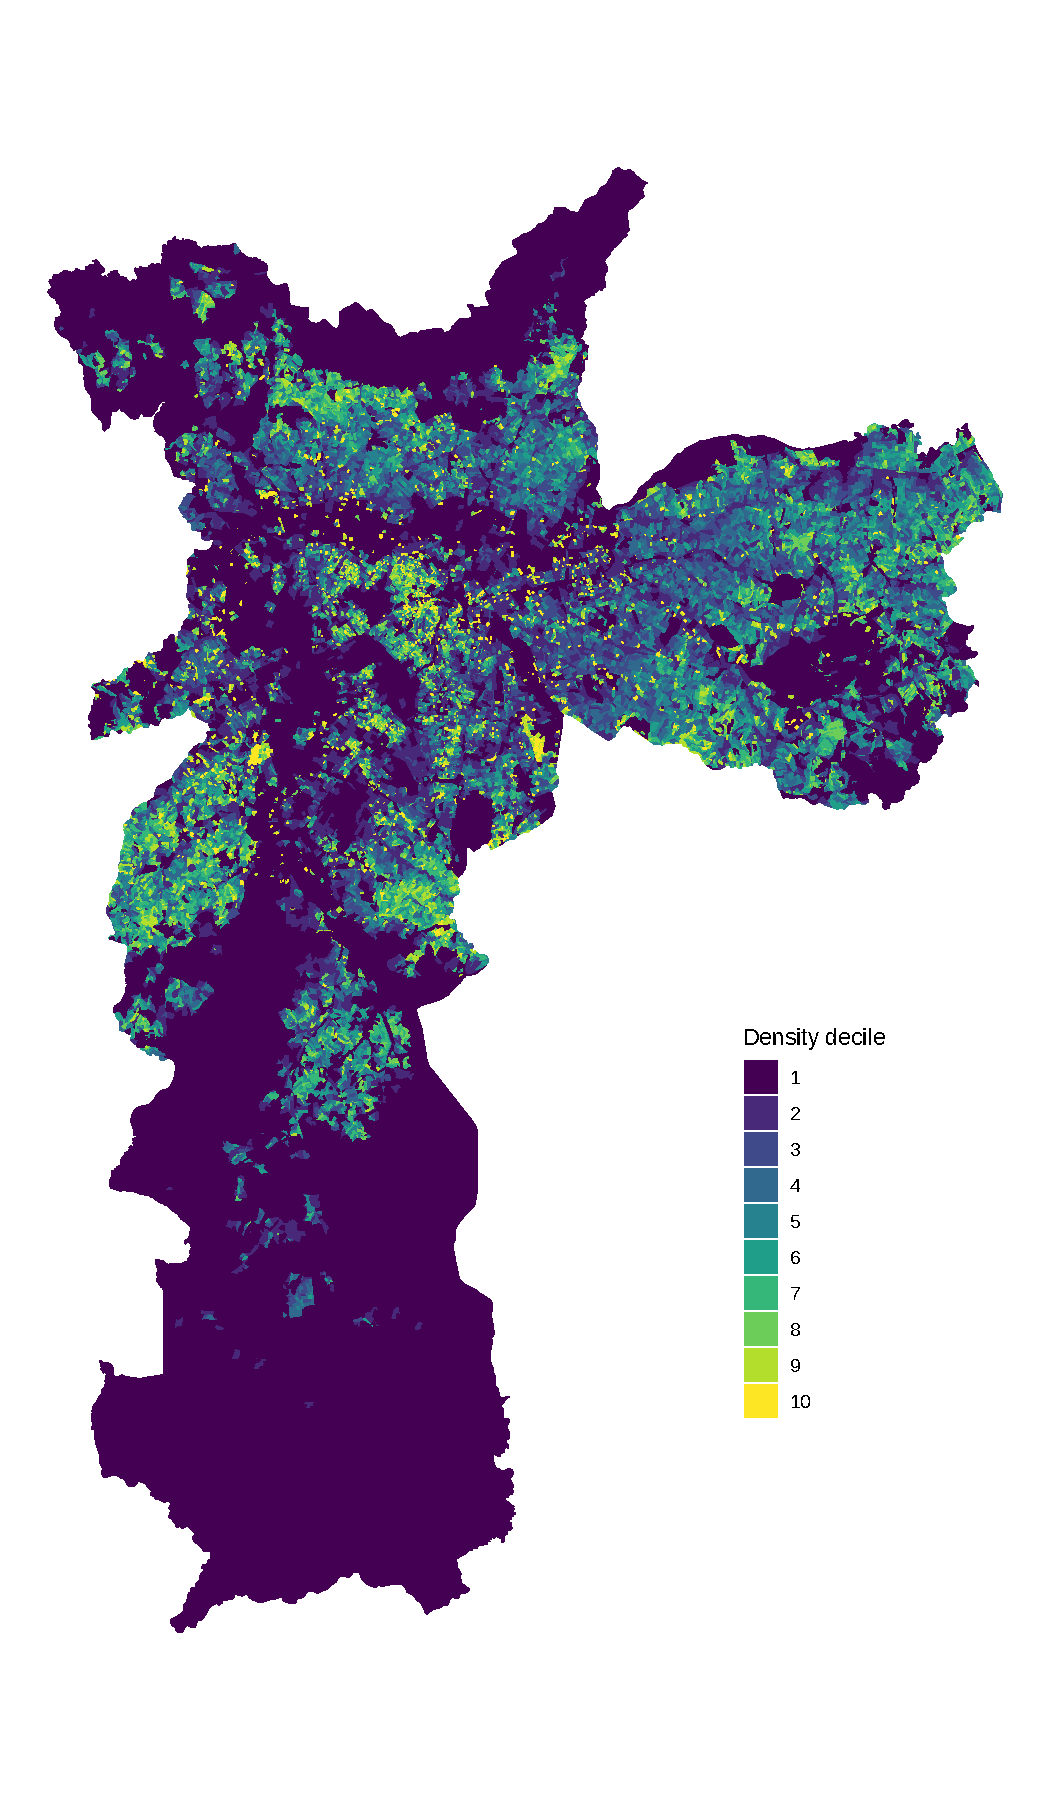
\includegraphics[width = .85\linewidth]{figuras/mapa-densidade.pdf}
    \label{fig:populacao}
\end{figure}


\begin{figure}[!h]
    \centering
    \caption{Regiões de eixos (pintadas em azul)}
    \includegraphics[width = .85\linewidth]{figuras/macroareas-eixos.pdf}
    \label{fig:eixos}
\end{figure}

\clearpage

\begin{figure}[!h]
    \centering
    \caption{Distribuição da quantidade de moradores em cada célula do raster}
    \includegraphics[width = .85\linewidth]{figuras/populacao-distribuicao-raster.pdf}
    \label{fig:populacao-rasters}
\end{figure}

\clearpage

\begin{figure}[!h]
    \centering
    \caption{Robustez dos resultados da regressão para diferentes espectros de irregularidade}
    \includegraphics[width = \linewidth]{figuras/robustez-regressao1pop.pdf}
    \label{fig:robustez-reg1}
\end{figure}

\end{apendicesenv}
    
    